\documentclass[
	12pt,				         				% tamanho da fonte
	openany,			     				% openright - capítulos começam em pág ímpar (insere página vazia caso preciso)
	chapter=TITLE,   				% títulos de capítulos convertidos em letras maiúsculas
	sumario=abnt-6027-2012, %tradicional, 
	oneside,			        				% twoside para impressão em verso e anverso. Oposto a oneside
	a4paper,			    				% tamanho do papel. 
	brazil,		         					% idioma adicional para hifenização
	english			        				% o último idioma é o principal do documento
	]{abntex2}

% Pacotes básicos 
\usepackage{lmodern}			% Usa a fonte Latin Modern			
\usepackage[T1]{fontenc}		% Selecao de codigos de fonte.
\usepackage[utf8]{inputenc}		% Codificacao do documento (conversão automática dos acentos)
\usepackage{lastpage}			% Usado pela Ficha catalográfica
\usepackage{indentfirst}		% Indenta o primeiro parágrafo de cada seção.
\usepackage{color}				% Controle das cores
\usepackage{graphicx}			% Inclusão de gráficos
\usepackage{microtype} 			% para melhorias de justificação
\usepackage{unijui}
\usepackage{enumitem}
\usepackage{tocloft}
\usepackage{leading}

\settocdepth{section}
 
\setlength{\cftsectionindent}{20mm}
\setlength{\cftsectionnumwidth}{10mm} 
\setlength{\cftsubsectionindent}{30mm}
\setlength{\cftsubsectionnumwidth}{10mm}


% Pacotes adicionais, usados apenas no âmbito do Modelo Canônico do abnteX2
\usepackage{lipsum}				% para geração de dummy text

% Pacotes de citações
\usepackage[english,hyperpageref]{backref}	 % Paginas com as citações na bibl
\usepackage[alf]{abntex2cite}	% Citações padrão ABNT

% CONFIGURAÇÕES DE PACOTES

% Configurações do pacote backref
% Usado sem a opção hyperpageref de backref
\renewcommand{\backrefpagesname}{Cited on page (s):~}
% Texto padrão antes do número das páginas
\renewcommand{\backref}{}
% Define os textos da citação
\renewcommand*{\backrefalt}[4]{
	\ifcase #1 %
		No citation in the text.%
	\or
		Cited on page #2.%
	\else
		Cited #1 times on pages #2.%
	\fi}%
    
%% adjusts names from abnTeX2
\addto\captionsenglish{% ingles
\renewcommand{\bibname}{References}
\renewcommand{\indexname}{Summary}
\renewcommand{\folhaderostoname}{Title page}
\renewcommand{\epigraphname}{Epigraph}
\renewcommand{\dedicatorianame}{Dedication}
\renewcommand{\errataname}{Errata sheet}
\renewcommand{\agradecimentosname}{Acknowledgements}
\renewcommand{\anexoname}{ANNEX}
\renewcommand{\anexosname}{Annex}
\renewcommand{\apendicename}{APPENDIX}
\renewcommand{\apendicesname}{Appendix}
\renewcommand{\orientadorname}{Supervisor:}
\renewcommand{\coorientadorname}{Co-supervisor:}
\renewcommand{\folhadeaprovacaoname}{Approval}
\renewcommand{\resumoname}{Abstract}
\renewcommand{\listadesiglasname}{List of abbreviations and acronyms}
\renewcommand{\listadesimbolosname}{List of symbols}
\renewcommand{\fontename}{Source}
\renewcommand{\notaname}{Note}
%% adjusts names used by \autoref
\renewcommand{\pageautorefname}{page}
\renewcommand{\sectionautorefname}{section}
\renewcommand{\subsectionautorefname}{subsection}
\renewcommand{\subsubsectionautorefname}{subsubsection}
\renewcommand{\paragraphautorefname}{subsubsubsection}
}

% Informações de dados para capa:
%\leading{8pt}
\titulo{A Hybrid Execution Model for a Runtime System to Execute Integration Processes for Business Intelligence in the Cloud Computing}
\autor{Student:\\ Daniela Freire Sellaro}
%\leading{10pt}

\local{Ijuí, RS, Brazil}
\data{2017}

\orientador{Dr. Rafael Zancan Frantz}

\coorientador{Dr. Inmaculada Hernández Salmerón \\
University of Seville (Spain)}

\tipotrabalho{Thesis Proposal}
%\leading{8pt}
\instituicao{Unijuí University \\
Department of Exact Sciences and Engineering \\
Postgraduate Program in Mathematical Modelling \\
Applied Computing Research Group    
  \par
}
\leading{16pt}
% Configurações de aparência do PDF final
% alterando o aspecto da cor azul
\definecolor{blue}{RGB}{41,5,195}

% informações do PDF
\makeatletter
\hypersetup{
     	%pagebackref=true,
		pdftitle={\@title}, 
		pdfauthor={\@author},
    	pdfsubject={\imprimirpreambulo},
	    pdfcreator={LaTeX with abnTeX2},
		pdfkeywords={abnt}{latex}{abntex}{abntex2}{trabalho acadêmico}, 
		colorlinks=true,       		% false: boxed links; true: colored links
    	linkcolor=blue,          	% color of internal links
    	citecolor=blue,        		% color of links to bibliography
    	filecolor=magenta,      		% color of file links
		urlcolor=blue,
		bookmarksdepth=4
}
\makeatother
 
% Espaçamentos entre linhas e parágrafos 
% O tamanho do parágrafo é dado por:
\setlength{\parindent}{1.3cm}

% Controle do espaçamento entre um parágrafo e outro:
\setlength{\parskip}{0.2cm}  % tente também \onelineskip

% compila o indice
\makeindex
% ---

% Início do documento
\begin{document}
\selectlanguage{english}
% Retira espaço extra obsoleto entre as frases.
\frenchspacing 

% Capa
\imprimircapa

% % Resumo em português:
% \setlength{\absparsep}{18pt} % ajusta o espaçamento dos parágrafos do resumo
% \begin{resumo}
% \label{sec:resumo}

Insira aqui o texto do resumo em português.

\textbf{Palavras-chaves}: Insira aqui as palavras-chave em português.
% \end{resumo}

% Resumo em inglês:
\begin{resumo}[Summary]
 \begin{otherlanguage*}{english}
\label{sec:abstract}

Companies are taking advantage of cloud computing to improve their business processes. The cloud computing requires the interaction with many kinds of applications, so it is necessary to improve the performance of software tools that allow keeping information on all these applications consistent and synchronised. Integration platforms are specialised software tools that provide support to design, implement, run, and monitor integration solution. The runtime system is the part of the integration platform responsible for running integration solutions.
Integration platforms, available as iPaaS services, consist of the same platforms designed and implemented for use on on-premise applications, merely encapsulated with a web interface and a few new adapters for connecting applications to the cloud or with cloud services. Therefore, runtime systems need to be adapted to the context of cloud computing, mainly seeking an increase in its performance and an optimization of the consumption of computational resources. 
This proposal presents research problems of the doctoral thesis and how they will be addressed, in order to contribute to migrate and adapt integration technologies to the context of cloud computing.
 \end{otherlanguage*}
\end{resumo}

% Sumário:
\pdfbookmark[0]{\contentsname}{toc}
\tableofcontents*
\cleardoublepage

\textual

% Introdução:
\chapter{INTRODUCTION}
%Introdução
This proposal presents the plan of work to the development of the thesis of doctoral of the Postgraduate Program in Mathematical Modelling, from the Unijuí University. The research is being carried out in the the Applied Computing Research Group (GCA), which is comprised of undergraduate, master and doctoral students and professors of Unijuí University, with the collaboration of others institutions. This research is supported by the Brazilian Coordination for the Improvement of Higher Education Personnel (CAPES/PROSUP).

Next, they are presenting the context of the field of study of enterprise application integration and cloud computing, the problem that motivates this research, the objectives pursued, our contributions to date and the important collaborations that this research has received. The following sections seek to provide detailed information about the research being developed over 48 months.
% \section{Identification}
% \begin{description} 
% \item [Nome:] Daniela Freire Sellaro
% \item [Thesis supervisor:] Dr. Rafael Zancan Frantz
% \item [Affiliation of supervisor] Department of Exact Sciences and Engineering of Unijuí University - Brazil.
% \item [Joint supervisor:] Dr. Inmaculada Hernández Salmerón
% \item [Affiliation of joint supervisor] Department of Languages and Information Systems of the University of Seville - Spain
% \item [Research line:] Computational modelling, optimization and systems control
% \end{description}
%**********************************************************************************************************************************
\section{Research Context}

%-- Context
\noindent 
Companies often need to use their software ecosystems~\cite{messerschmitt:2005} to support and improve their business processes. These ecosystems are composed of many applications, usually designed without taking into account their possible integration. Within the area of Software Engineering, the field of studies known as Enterprise Integration Applications (EAI)~\cite{frantz2016} seek to provide methodologies, techniques and tools for the design and implementation of integration solutions. In general terms, an integration solution aims to orchestrate a set of applications to keep them synchronized or provide new features that can be built from those already developed. An integration solution is composed of processes that contain the integration logic and ports that encapsulate adapters for communication protocols, which connect ecosystem processes or applications to the integration solution.

Integration platforms are specialised software tools that provide support to design, implement, run, and monitor integration solution. 
In the last years, many integration platforms have been created by the EAI community. These platforms have been heavily influenced by the catalogue of conceptual integration standards documented by Hohpe and Woolf~\cite{hohpe2004} and adopt the architectural style of pipes-and-filters~\cite{alexander1977}. In an integration solution, pipes represent message channels, and filters represent atomic tasks that implement a concrete integration pattern to process encapsulated data in messages. The adoption of this architecture allows to unsynchronised the tasks that make up the integration solution.

There are several open source platforms that can be used to build integration solutions such as Mule~\cite{dossot2014}, Camel~\cite{isen2010}, Spring Integration~\cite{fisher2012}, Synapse~\cite{rademakers2008,jayasinghe2011}, Fuse~\cite{russell2012}, ServiceMix~\cite{konsek2013}, Petals~\cite{surhone2010}, Jitterbit~\cite{russell2012_1}, WSO2 ESB~\cite{indrasiri2016} and Guaraná~\cite{frantz2012}. Usually, these integration platforms provide a domain-specific language, development toolkit, test environment, monitoring tool, and runtime system. The domain-specific language is focused on the elaboration of conceptual models for the integration solution, with a level of abstraction close to the domain of the problem. The development kit is a set of software tools that allows the implementation of the solution, that is, the transformation of the conceptual model to the executable code. The testing environment allows testing individual parts or the entire integration solution, with the aim of identifying and eliminating possible defects in the implementation of the same. The monitoring tool is used to monitor, at runtime, the operation of the integration solution and detect errors that may occur during message processing. The runtime system provides all the support required to run these integration solutions.

Cloud Computing~\cite{NIST:2011} is another field of studies that has drawn the attention of the scientific community and represents a new paradigm of development, commercialization and use of software. This field has been transforming the current software ecosystems and revolutionizing the way companies provide computer support to their business processes. Cloud computing enables companies to contract service packages by dramatically reducing their total cost of ownership (TCO) with the information technology (IT) infrastructure, without sacrificing the quality of the IT support provided to their business processes. This is due mainly to the pay-as-you-go charging model that allows users to rate cloud computing based on the amount of computing resources consumed~\cite{buyya:2009,SOUSA:2009}. Along with the pay-as-you-go model, cloud computing has also brought the elasticity feature, which allows for incremental and decreasing computational resources to better meet the demands of applications running on the cloud infrastructure~\cite{DIAS:2015}.
The advancement of cloud computing technologies has led companies to a major transformation in their software ecosystem, which now includes on-premise applications, migrated applications for virtual machines in the cloud, social media applications and many other software services available in the cloud. 

% %-- Our solution
This research proposal presents the properties study that can have an impact on the performance of runtime system, regarding the ability to process messages efficiently and ensure a fair execution of tasks. runtime systems of popular integration platforms were evaluated regarding theses proprieties and it was observed that they are not sufficiently adapted to the context of the cloud computing. After, the research problems, that will contribute to migrate and adapt integration technologies to this context, are presented.
%**********************************************************************************************************************************
\section{Motivation}

%-- What is the problem? 
The quality of service, that integration solutions are able to achieve in terms of message processing, is directly related to the runtime system the integration platform. Typically, in order to achieve the desired quality of service with an integration solution, software engineers have increased computational resources in the server machine on which the integration platform is installed within the enterprise. This approach links the increased performance of an integration solution to the increase in financial costs required to augment the current hardware or the purchase of a new server with greater processing power that can generate the desired impact on the performance of the runtime systems, thus increasing the number of messages processed by the integration solutions.
The hiring of virtual machines in the cloud to host the integration platforms allows a reduction of the total cost of ownership for the realization of the EAI by the companies, as well as through the feature of elasticity of the cloud, a greater flexibility for the increment of computational resources.

This has led companies to want to migrate integration platforms and run their integration solutions in the cloud. The migration of integration platforms to virtual machines in the cloud has given rise to a new service model that is being referred to by the EAI community as integration Platform-as-a-Service (iPaaS)~\cite{pezzini2011}. Data from 2015 show that, together, Latin America, Central America and North America account for 67\% of the market for iPaaS integration platforms, followed by Europe, the Middle East and Africa, which together account for 22\%, and Asia and the Pacific with 11\% of this market, and these values should remain, with little oscillation, by the end of 2019~\cite{sharma2015}. The traditional market for integration platforms used on-premise registered growth of less than 10\% in 2016, while the market for iPaaS integration platforms had a 60\% expansion over the previous year, representing a global market of 700 million Dollars~\cite{guttridge2017}. As early as 2017, two out of three application integration projects are developed directly with cloud integration platforms~\cite{pezzini2015}. The investment made by companies in iPaaS integration platforms will increase by 40\% by 2019~\cite{sharma2015}, making iPaaS the preferred integration platform by companies and with annual revenue growth higher than the traditional platform market of integration used on-premise~\cite{guttridge2017,sharma2017}.

%-- % %-- Why it is a problem?
Given the high investments in iPaaS integration platforms, a research effort is needed to study and adapt these platforms to the new paradigm that represents cloud computing. In this context, the efficiency of runtime systems is fundamental since a number of computing resources in the cloud follows the pay-as-you-go model, and therefore has a direct impact on the financial cost involved in executing the solutions. The higher the efficiency of runtime systems, the less computational resources will need to be contracted or consumed in order for an integration solution to achieve the expected quality of service. In this proposal, performance is defined as the ability to process more messages per unit of time, without having to increase the number of computational resources allocated to the runtime system.
%**********************************************************************************************************************************
\section{Objectives}

\subsection{Main}

Reduce the average processing time of a message through the integration process, considering concurrently the optimization of the threads needed in this process.

\subsection{Specific}

\begin{enumerate}%[label=(\alph*)]
    \item Develop of a comparison framework for integration runtime system.
    \item Develop a modelling for a runtime system more efficient.
    \item Develop a prototype for a runtime system more efficient.
	\item Minimize the following variables:
    \begin{itemize}
    	\item thread management time, in relation to the creation, destruction and context change of them;
		\item waiting time of a task in the ready queues.
		\item task processing time;
    	\item time gap between a task becomes ready to execute and its execution completion.
    \end{itemize}
	\item Maximizing the total amount of messages processed by the integration process per time unit.
		\item Avoid thread concentration in the initial tasks of the integration flow in the task queue when there is an increase in the incoming message load.
	\end{enumerate}
    
%***********************************************************************************************************************************
\section{Contributions}
\label{sec:contributions}  
\noindent

This section brings the main contributions to date. 
     
\subsubsection*{Articles submitted to international journal:}

\begin{itemize}
\item \textit{Towards a Methodology to Compare Enterprise Application Integration Platforms Focusing on Performance.}

At: Software Practice and Experience. Qualis: A2. JCR: 1.60;
\item \textit{A Survey on the Runtime Systems of Enterprise Application Integration Platforms Focusing on Performance.}

At: Journal of Systems and Software. Qualis: A2. JCR: 2.44;
\item \textit{Optimization of the size of thread pool in runtime systems to Enterprise Application Integration - a mathematical modelling.}

At: Computational and Applied Mathematics. Qualis: B1. JCR: 0.96;
\item \textit{Novel Task Scheduling Proposal to Runtime System Integration Platforms.}

At: Journal of Systems and Software. Qualis: A2. JCR: 2.44
\end{itemize}

\subsubsection*{Articles presented in conference:}
\begin{itemize}
\item \textit{Task Scheduling Optimization on Enterprise Application Integration Platforms Based on the Meta-heuristic Particle Swarm Optimization}

At: XXXI Simpósio Brasileiro de Engenharia de Software (SBES) Qualis: B2.
\end{itemize}

\subsubsection*{Articles published in workshops:}

\begin{itemize}
\item \textit{Execução de Soluções de Integração de Aplicações Empresariais na Nuvem: Perspectivas e Desafios}

At: IV Seminário de Formação Científica e Tecnológica (SFCT), Ijuí, Brazil.
\end{itemize}

%**********************************************************************************************************************************
\section{Collaboration in Research}  
\label{sec:collaboration}  
\noindent

This research counts on collaborations with the following researchers:

\begin{itemize}
\item Dr. Fabricia Roos-Frantz (Unijuí University, Brazil): participation in follow-up meetings and seminars, feedbacks about our inferences, articles review, assistance in the field of study of scientific methodology and software engineering.
\item Dr. Sandro Sawicki (Unijuí University, Brazil): participation in follow-up meetings and seminars, feedbacks about our inferences, articles review, help in the field of study of optimization techniques.
\item Dr. Vitor Manuel Basto Fernandes (University Institute of Lisbon, Portugal): participation in follow-up meetings and seminars, feedbacks about our inferences, articles review, help in the field of study of data science.
\item Dr. Inmaculada Hernández Salmerón (University of Seville, Spain): participation in follow-up meetings and seminars, articles review, feedbacks about our inferences, help in the field of study of cloud computing.
\item Dr. Rafael Corchuelo (University of Seville, Spain): planning of steps of the research, planning, definition of research problems, participation in follow-up meetings and seminars, articles review, feedbacks about our inferences.
\end{itemize}
%
% Others institutions that collaborate with GCA, by means of participation in coordinated projects, joint directions, joint publications, research visits:
% \begin{itemize}
% \item Cambridge University (United Kingdom) 
% \item Rochester Institute of Technology (United States)
% \item De Montfort University (United Kingdom) 
% \item Leiden University (Netherlands) 
% \item Federal University of Rio Grande do Sul (Brazil) 
% \item Federal University of Rio de Janeiro (Brazil).
% \end{itemize}

%**********************************************************************************************************************************

\section{Structure of this Document}  
\noindent

The rest of this proposal is organised as follows: Section~\ref{cap:methodology} presents the methodology; Section~\ref{cap:stateofart} presents the technical and scientific literature review about integration platform; Section~\ref{cap:researchproblems} lists the issues to investigated derived of the literature review; Section~\ref{cap:validation} reports how results will be judged, interpreted and validated; Section~\ref{cap:schedule} shows a time-table for achieving key objectives, plans in cases where goals are not met by specific target date and informers the current state of the research; and Section~\ref{cap:infrastructure} describes the infrastructure available to develop this research.

%
% % Capítulo 2:
% \chapter{STATEMENT AND OBJECTIVES}
% \input{src/objectives.tex}
% Capítulo 2:
\chapter{METHODOLOGY}
%capitulo04
\label{cap:methodology}
\noindent 
The project is divided into cycles, in which a set of activities must be performed. At the beginning of each cycle, a planning meeting is held, in which supervisor together with the proponent define and prioritize the points that will be worked during the cycle, select the activities that must be implemented and the products or artefacts that will result from the work done during that cycle.

At the end of each cycle, the proponent presents the progress of the work, through a meeting or seminar, depending on the relevance of the work done for the research progress. In such meetings, besides being a supervisor and a coordinator, GCA teachers and students will be able to participate, in person and through video conference. The objective is to promote discussions, disseminate knowledge, identify possible inconsistencies and collect new ideas about the work carried out in the cycle that ends. 

As the research progresses and incremental content is generated, the proponent participates in workshops and conferences to discuss ideas and have feedback. When these research increments are complete and mature, they are published in journals for dissemination of the results.
In addition, at the end of the cycle, the proponent and her supervisor will hold an evaluation meeting to assess the timing, productivity, learning and planning of the next cycle.
Then a new one begins, repeating the process until the whole schedule presented in Section~\ref{cap:schedule} is fulfilled.

It is worth mentioning that one of the artefacts that will be generated at the end of the cycle will be the research report, which will have periodicity defined by the supervisor.
It is also important to highlight that the GCA is formed by professors of several institutions, which are listed in the Section~\ref{sec:collaboration}. Their researches belong to different fields of research within Software Engineering, with emphasis on the Enterprise Application Integration, under which this project is anchored.

It is the intention of the proponent and her advisor that part of the research is carried out in the laboratory of the TDG Seville group, at the University of Seville in the Spain, under the supervision of Professor Dr. Inmaculada Hernández Salmerón, linked to this university. This exchange will strengthen the international collaboration activities of the Postgraduate Program in Mathematical Modeling of UNIJUI with the postgraduate program of the University of Seville and it will have the duration of one year, probably between April 2018 and March 2019, according to the schedule.
\clearpage
The research can be divided into seven major steps:
\begin{enumerate}
\item Research Context review. 

This first step of the research consisted in the study of the research context, including EAI, runtime system, cloud computing and big data. In this phase, the study was accompanied by meetings, seminars, which solidified the knowledge gained.
\item Literature review. 

This step of the research was the to deepening in the fields: enterprise application integration, runtime system, cloud computing, big data, mathematical modelling, optimization techniques, statistics models and multithread programming. The databases utilized in this research are IEEE Xplore, ACM Digital Library, Scorpus. In this phase, There was production of articles, which resulted in good feedbacks.
\item Technical and scientific literature review.

This step of the research consisted of studying runtime systems from known integration platforms. Properties that may have an impact on the performance of runtime systems were identified and from these properties, weaknesses of the runtime systems studied were also identified. The research problems that will be approached in this thesis derived from the identification of these weaknesses.
\item Proposal modelling.

In this step, alternatives for runtime systems are studied: \textit{(i)} to take advantage of the parallel programming of multiprocessors; (ii) create and configure thread pool dynamically and elastically, following the demand for tasks; (iii) has a more optimized scheduling of tasks for the thread pools; \textit{(iv)} have mechanisms to detect bottlenecks in the execution of integration solutions; \textit{(v)} knows the computational complexity of the tasks being executed.

\item Development of a prototype.

In this step, a proof of concept to measure the gains of the proposed runtime system will develop.
\item Validation of the proposal.

In this step, statistical validation described in Section~\ref{cap:validation} will carry out.
\item Thesis writing.

The last stage contemplates the closing of the works, evaluation of the obtained results and writing the thesis. 
\end{enumerate}

% Capítulo 3:
\chapter{STATE OF THE ART}
%capitulo02
\label{cap:stateofart}
\noindent 
This section presents our research of the integration platforms under the perspective of the performance of the runtime systems. The technical and scientific literature were reviewed from a set of properties that can have an impact on the performance of runtime system, such properties were classified in two dimensions: efficiency and fairness execution. The dimensions and their respective properties are detailed as follows.

%==============================================================================
\section{Efficiency}
\label{sec:efficiency}
%==============================================================================

This dimension relates to improving the efficiency of the runtime system to process a message, which can also be seen as increasing the average number of messages processed by time unit. It comprises the following properties that relates to the capacity of reducing the real time demanded by the integration solution to completely process a message:
\begin{itemize} 
\item \textbf{Designed for Multi-core}. Multi-core programming has to be carried out in order to take full advantage of multiple cores available in the hardware processors. This property indicates whether the runtime system has been developed to take advantage of multi-core or not. Multiple cores work together to increase the capability of process multiple tasks or increase the performance of the system by operating on multiple instructions simultaneously in an efficient manner. It can take the following values: \texttt{yes} or \texttt{no}. \texttt{yes} indicates the runtime system was developed to take advantage of multi-core hardware, otherwise, the value is \texttt{no}.

\item \textbf{Thread Pool Configuration}. The runtime system allows to configure one or more pools of threads to the integration solution, and this property indicates how threads are managed in these pools. This property may take the following values: \texttt{fixed}, \texttt{limited} or \texttt{elastic}. \texttt{fixed} indicates that a thread pool is composed of a fixed number of threads, which is known at design time; \texttt{limited} indicates the number of threads in a thread pool can increase automatically during runtime until a threshold defined at design time is reached; \texttt{elastic} indicates that the number of threads in a thread pool can automatically increase and decrease during runtime within a range of values defined at design time.
%
\item \textbf{Type of Message Storage in Process}. Messages can contain a huge amount of data, which will have an impact on the amount of memory required by channels inside the integration solution and depending on the type of storage it has an impact on the real time execution. This property indicates whether the message is stored in memory, disk, or both. It may take the following values: \texttt{in memory}, or \texttt{in disk}, or \texttt{in memory \& disk}.
%
\item \textbf{Distributed Process Execution}. Indicates whether an integration solution can be divided and distributed to different machines to execute a set of correlated messages, promoting scalability. This property allows increasing the number of tasks executed per time unit in cases in which there is no dependency between the tasks, i.e., the input data of one task is the output data produced by another task. This property may take the following values: \texttt{yes} or \texttt{no}. \texttt{yes} indicates the runtime system takes advantage of scalability, otherwise, the value is \texttt{no}.
%	
\item \textbf{Thread Pool Creation}. Historical and current execution data can be used by runtime systems to make decisions during runtime, determining optimised strategies to create threads. This property indicates the way and stage at which thread pools can be created. This property may take the following values: \texttt{dynamic} or \texttt{static}. \texttt{dynamic} indicates that thread pool creation is done at runtime from data taken from the runtime system and indicates the need for a pool and \texttt{static} value indicates that the pool creation is done at design time by the software engineer.	
\end{itemize}
%
%==============================================================================
\section{Fairness execution}
\label{sec:fairness}
%==============================================================================

This dimension concerns to assignment of threads to tasks aiming at a fair execution of them to help to minimise the average time that a message takes to be processed in the integration solution. The following properties provide means that contribute to have a fair execution of tasks:
\begin{itemize}
% 	\item \textbf{Priority to task execution}. Indicates whether the runtime system allows tasks to have priority associated with them so that it affects the execution policy by the runtime system. This property may take the following values: \texttt{yes} or \texttt{no}. \texttt{yes} indicates the runtime system can deal with priority in tasks.
%	
\item \textbf{Starvation Detection}. Indicates whether the runtime system is endowed with the capacity to detect tasks that do not execute within an accepted time-frame. This property may take the following values: \texttt{yes} or \texttt{no}. \texttt{yes} indicates the runtime system can detect starvation, otherwise, the value is \texttt{no}. 
%	
\item \textbf{Thread Pool Policy}. Indicates the strategy followed by the runtime system to assign the existing threads to the different tasks. This property may take the following values: \texttt{FIFO}, \texttt{priority} or \texttt{mapping}. \texttt{FIFO} means that the runtime system follows First-In-First-Out(FIFO) heuristic, in which the threads are being allocated the tasks in order that arrive, so that the first ones that arrive are attended to before; \texttt{priority} means that the runtime system allows tasks to have priority associated; and, \texttt{mapping} means that the scheduling policy follows a mapping based on a mathematical model or optimization method that allows finding an optimal scheduling policy by previously evaluating the integration solution.
%	
\item \textbf{Task Complexity}. Indicates whether the runtime system takes into consideration the computational complexity of tasks to allocate threads. This property may take the following values: \texttt{yes} or \texttt{no}. \texttt{yes} indicates that the runtime system knows the computational complexity of each of the tasks and this can be utilised in the decision in choosing the order of execution of tasks, such as tasks of less computational complexity can be executed first, as soon as possible; otherwise, the value is \texttt{no}.
%
\item \textbf{Execution Model}. Indicates the execution model implemented by the runtime system, which deals with the granularity of the execution of tasks. This property may take the following values: \texttt{process-based}, \texttt{task-based} or \texttt{hybrid}. In the \texttt{process-based} model, the runtime system controls process instances as a whole, i.e., there are no means that it can interact with the internal tasks; contrarily, in the \texttt{task-based} model, the runtime system may control both process instances and their internal tasks. In the \texttt{hybrid} model, the runtime system will adopt the model that better fits the execution profile about some predefined parameters, such as message input rate, the number of processors, average message size. 
%
\item \textbf{Throttling Controller}. Indicates whether the runtime system allows controlling the rate of incoming messages on input ports. If the input rate exceeds the processing capacity of the initial tasks, the runtime system can adopt suitable policies, such as, refusing new messages on passive ports or tuning the frequency of the pooling in the active ports. This property may take the following values: \texttt{yes} or \texttt{no}. \texttt{yes} indicates that the runtime system can control the rate of incoming messages, that is, it has a throttling controller; otherwise, the value is \texttt{no}. 
\end{itemize}
%==============================================================================
\section{Analysis and Discussion}
\label{sec:analysis}
%==============================================================================

We selection some popular integration platforms to analyse the values of the described proprieties. For this, we rely in the methodology the integrative literature review, which includes the following steps: identification of the theme and elaboration of the inclusion and exclusion criteria of articles, construction of an instrument for collection of relevant data of the articles found, evaluation and analysis of the articles selected in the research, interpretation and discussion of the results obtained and presentation of the review.

We search the databases: IEEE Xplore, ACM Digital Library, Scorpus, using the keywords: "runtime system" and "execution engine". The inclusion criteria were: articles published in English, abstracts available in the chosen databases, availability of the same in full, published between the period from 2012 to 2017, not to restrict the area of knowledge used by the runtime systems.
We revised the Gartner report~\cite{gartner2016,guttridge2017} and Ovum report~\cite{sharma2017} for integration platforms and also made an exhausting search on the Web to build a list of candidate integration platforms. 

We have adopted the following criteria to select the integration platforms: they must follow the pipes-and-filters architectural style~\cite{alexander1977} and support enterprise integration patterns (EIPs)~\cite{hohpe2004}.
%and have their code under an open source license. 
The pipes-and-filters architecture style suggests dividing a task into smaller tasks, which are connected through communication channels in the message flow of the application, and the output of one task is the input to the next. In this architectural style, the computational components that perform an atomic task on inbound messages to route, transform or modify them and produce one or more outbound messages which are sent to the next filter by means of a communication channel, called pipe. We apply the aforementioned criteria and then we exclude those that did not meet the criteria or had not enough documentation to infer the values of the properties.

Enterprise integration patterns are conceptual standards identified and documented by Hohpe and Woolf~\cite{hohpe2004}, such standards have become a benchmark amongst software engineers and have inspired several integration platforms~\cite{isen2010,dossot2014,fisher2012,frantz2012}. EIPs document a set of best-practices to implement tasks which help to solve recurrent application integration problems.

We have analysed the runtime system of Mule~\cite{dossot2014}, Camel~\cite{isen2010}, Spring Integration~\cite{fisher2012}, Synapse~\cite{rademakers2008,jayasinghe2011}, Fuse~\cite{russell2012}, ServiceMix~\cite{konsek2013}, Petals ESB~\cite{surhone2010}, Jitterbit~\cite{russell2012_1} and WSO2 ESB~\cite{indrasiri2016}. It is important to note that the component SE Camel embeds the Apache Camel routing runtime system to execute enterprise integration patterns (EIP) in Fuse, ServiceMix and Petals, therefore, some properties have the same values.

The comparison of the runtime systems, regarding proprieties related to efficiency and fairness execution are summarised in Table~\ref{tab:comparison}.
\begin{table*}[htbp]
	\centering
	\caption{Comparison between runtime systems.}
    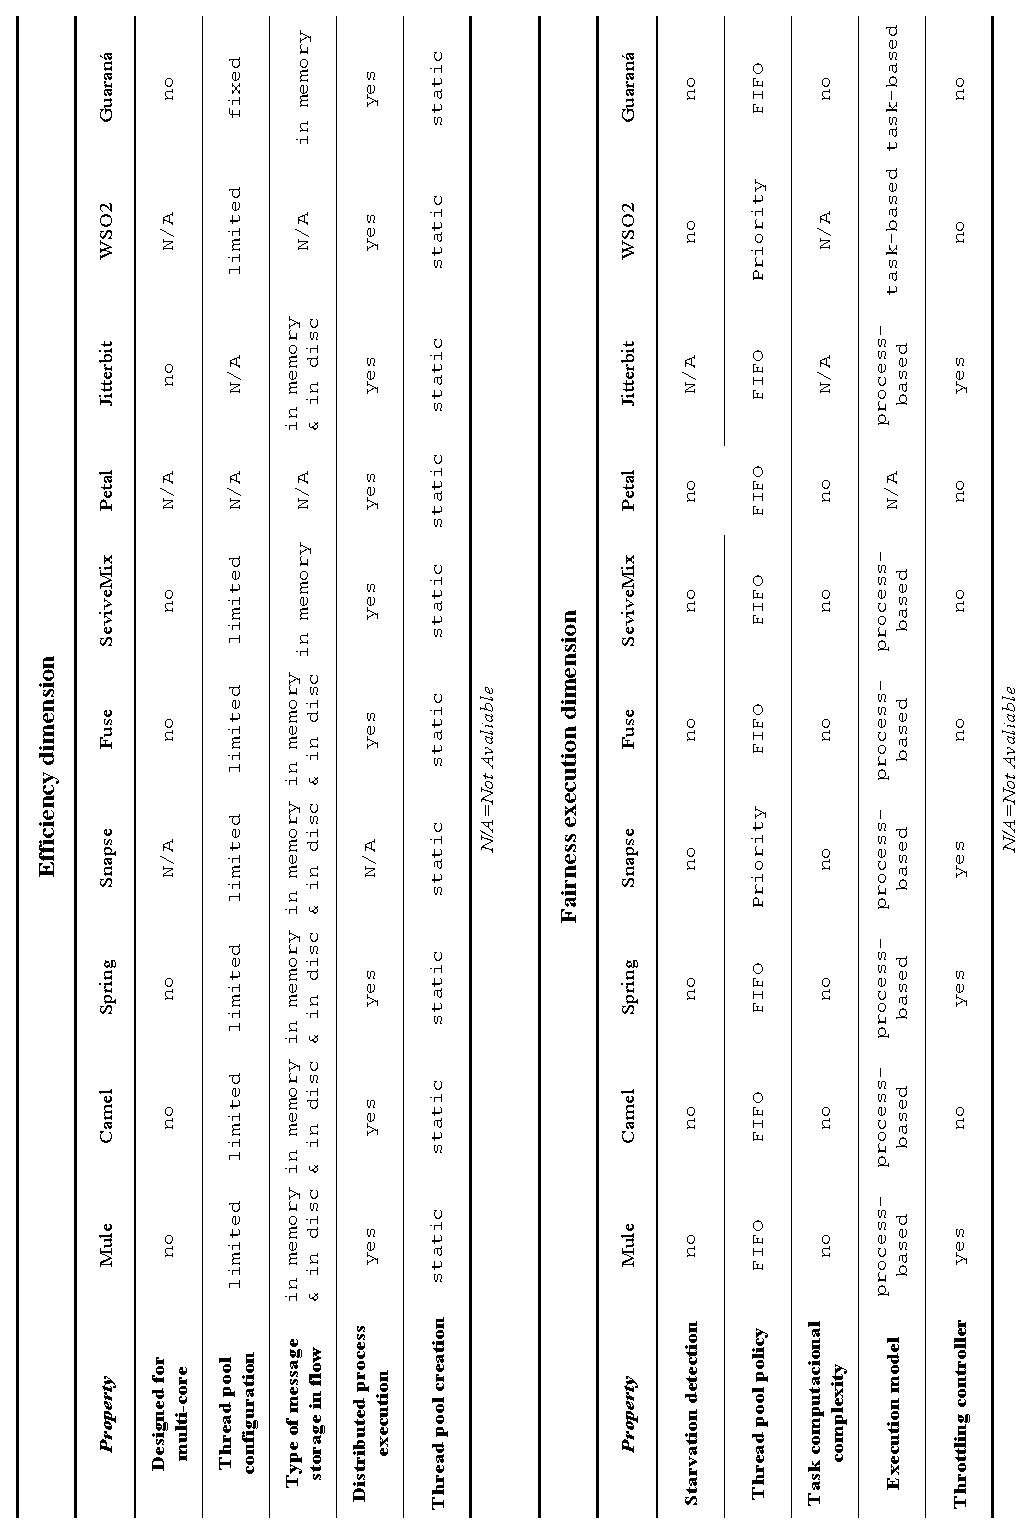
\includegraphics[scale=0.8]{./figs/table_dimensions_v.eps}
	%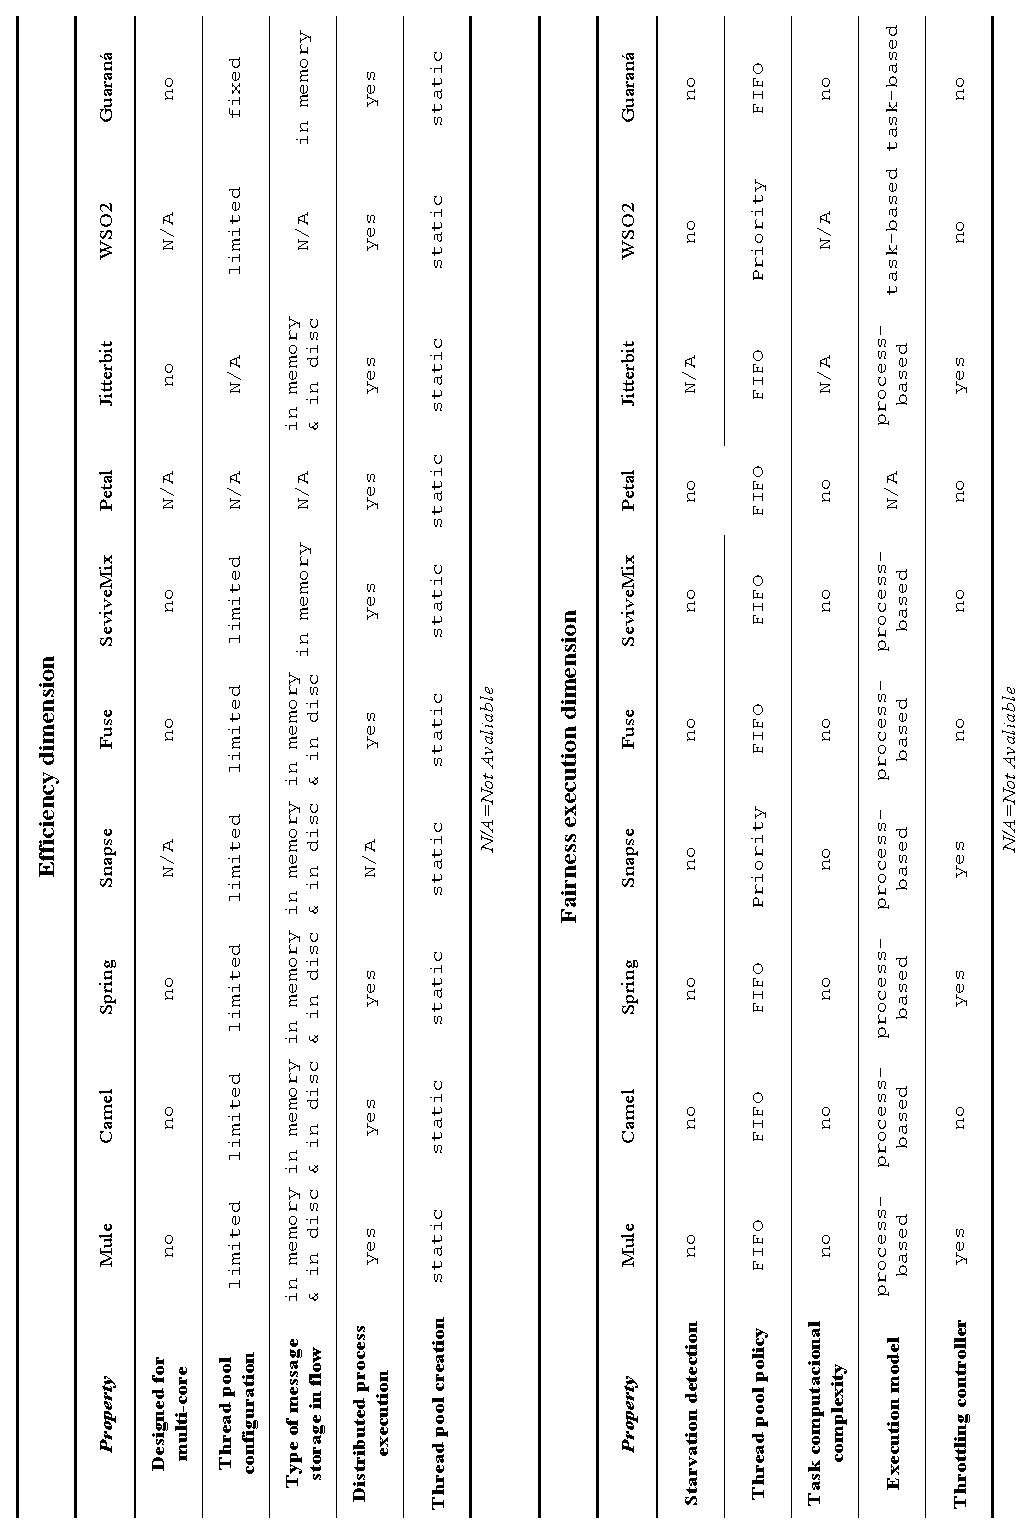
\includegraphics[width=\linewidth]{./figs/table_dimensions_v.eps}
	\label{tab:comparison}
\end{table*}

None of the integration platforms have their runtime system designed to take advantage of multi-core. Although, Mule, Camel and Jitterbit use some language resource for to implement the parallel programming, there not is information about proprieties of runtime systems that take advantage of physically tasks of an integration solution.

Every runtime systems have pools of threads which can increase or decrease the limited number of threads available to tasks, except Petals and Jitterbit, in which there is no information that allow us to evaluate them regarding this property; and Guaraná the provide a fixed pool of threads.

Mule, Camel, Spring Integration, Synapse, Fuse, ServiceMix and Jitterbit can deal with both common data, storing in memory, and big data, storing in disc. ServiceMix and WSO2, there is no information that allow us to evaluate them regarding this property, so we have assumed they, as well as Guaraná, store message only in memory.

The ability to distribute the execution of tasks amongst several virtual machines is present in every analysed runtime systems, except in Synapse, where there is no information that allow us to evaluate them regarding this property. 

None of these runtime systems is able to creation dynamically thread pool, optimising their task execution strategies from the analysis of the flow of messages in the integration solution. Petals, there is no information that allow us to evaluate it regarding this property, so we have assumed it do not provides creation dynamic thread pool.

The capacity to detect tasks that are not executed within an accepted time frame is absent in every analysed runtime systems, except for Jitterbit, there is no information that allow us to evaluate it regarding this starvation detection property. Every analysed runtime systems chose FIFO heuristic as strategy for tasks scheduling, except Synapse and WSO2 have a strategy for distinguish tasks, in order to influence their scheduling, that is, priority based. 

None runtime systems considers the computational complexity of tasks to allocate threads, except for Jitterbit and WSO2, there is no information that allow us to evaluate them regarding this property, so we have assumed they not have considering the computational complexity of tasks to allocate threads.

Every runtime system implement process-based execution model, in which the runtime system controls process instances as a whole, except Guaraná and WSO2 which implement task-based execution model; and Petals, there is no information that allow us to evaluate them regarding this property, so we have assumed they adopt process-based execution model. 

Mule, Spring, Synapse and Jitterbit allow to control the rate of incoming messages on incoming ports; the others have not throttling controller.

Mule, Camel and Jitterbit platforms present resources of parallel programming, but none of the analysed runtime systems are designed to take advantage of the physical cores of the processor.
Runtime systems are similar about pool threads configuration at tasks, however, none has the ability which allows runtime systems automatically increase and decrease to more efficiently meet demand peaks, as well as eliminate threads to release computational resources when they are no more necessary. 

In Mule, the threading profile specifies how the thread pools behave. It is possible to specify a separate threading profile for each input thread pool, flow thread pool, and output thread pool~\cite{Mule}. Camel and ServiceMix offer both a fine grained configuration where it is possible tweak individual pools and have more coarse grained configuration with fall back to global settings; furthermore, it should be possible to define a set of rules which matches, which thread pool a given source should use, task or group of task~\cite{Camel}. Every runtime system has classes which extends a class \texttt{ThreadPoolExecutor} of the language Java and their methods which set size pool, number maximum of thread in pool, amongst others. Camel and ServiceMix allow global settings pools, while Synapse and WSO2 have a property file, which contains global parameters for tuning its global pool of threads~\cite{WSO2}. 

Runtime systems are advanced in storing messages in flow. The ability of disk storage allows runtime systems to deal with big data~\cite{chen2014}, that is, larger data in size or volume. Usually, disk storage can increase the total time of message execution, so that it should be used in scenarios where this type of storage is really needed. Mule uses object stores to persist data for eventual retrieval. Internally, it uses object stores in various filters, routers, and other message processors that need to store state between messages. In most cases, Mule creates and manages object stores automatically, and provides two types of object stores: \texttt{In-memory store} and \texttt{Persistent store}. \texttt{In-memory store} are stores objects in local Mule runtime memory. Objects are lost on shut-down of Mule runtime. In \texttt{Persistent store}, Mule persists data when an object store is explicitly configured to be persistent. In a standalone Mule runtime, Mule creates a default persistent store in the file system~\cite{Mule}. 

Camel and ServiceMix allow to save the message in a persistent store: in a file or database~\cite{isen2010}. Spring Integration defines the \texttt{Message Store} pattern, which allows enterprise integration patterns (EIP) components to store messages typically in some type of persistent store, in addition to capability to buffer messages~\cite{Spring}. Synapse uses the Java classes: \texttt{AbstractMessageStore} and \texttt{InMemoryMessageStore} to store message in disc and in memory, respectively~\cite{Snapse}. Fuse offers a number of different persistence mechanisms besides the default message store, including: \texttt{KahaDB message store}, \texttt{distributed KahaDB}, \texttt{LevelDB} and \texttt{JDBC adapter}. The \emph{KahaDB Message Store} is the default message store uses a hybrid system that couples a transactional journal for message storage and a reference store for quick retrieval. The \texttt{distributed KahaDB} persistence adapter allows to distribute a destinations of broker across multiple \texttt{KahaDB message stores}. The \texttt{LevelDB message} store is a file based message store implemented using LevelDB of Google library to maintain indexes into log files holding the messages. Fuse supports the use of relational databases as a message store through JDBC, where it is possible persistence adapter either coupled with a high performance journal or standalone~\cite{Fuse}. Jitterbit is also able persist message to a file system~\cite{Jitterbit}.

Runtime systems are fit the cloud computing~\cite{hwang2013} environment in which processing can be distributed across multiple virtual machines, providing greater processing power for tasks that can be processed in parallel. However, it is important that the data transfer time from one machine to another minimises the total message processing time because if the total processing time increases, the distributed processing will be detrimental to the performance of the runtime system.

Mule has a virtual server composed of multiple nodes, which ensures high system availability, realising distributed process execution. To get high performance, it is possible configure a Mule cluster or an individual application for maximum performance using a performance profile. By implementing the performance profile for specific applications within a cluster, it is possible maximise the scalability of the deployments while deploying applications with different performance and reliability requirements in the same cluster~\cite{Mule}.

Camel, Fuse and ServiceMix propose different solutions to allow their solution to be scalable, to distribute the load between different instances, such as load balancing, clustering and cloud computing. The approach of the load balancing allows to distribute the load between different endpoints, which plays the role of a \textit{proxy}. The clustering can be achieved through work distribution, consumer competition, amongst others, depending of the infrastructure configuration: one or several instances running on the same machine or distribute across a cloud of servers. For cloud computing, it is possible to create a Cassandra endpoint to allow to consume or to push messages from Cassandra NOSQL database~\cite{Camel}. 

Spring Integration provides a consistent model for intraprocess and interprocess messaging implemented using Java Message Service(JMS)~\cite{fisher2012}. Petals distributes its processes in a static and dynamic way. In static, no new node can be added to a running Petals cluster. In dynamic, it is possible this distribution be updated regularly, so can add new nodes to a running Petals cluster~\cite{Petals}. Jitterbit includes a multi-tenant, auto-scaling agent group called \texttt{Jitterbit Cloud Agent Group}. Agent Groups provide for high availability and load balancing of integration operations across runtime servers within a group. In case of the \texttt{Cloud Agent Group}, it is automatically scaled within the cloud as necessary, and does not require adding runtime servers to expand capacity~\cite{Jitterbit}. 

WSO2 implements a distributed process by means of two models. The first model consists of two sub cluster domains as worker domain and management domain. These sub domains take up load according to a defined load balancing algorithm and auto-scales according to the load on its nodes. The second model consists of a single cluster, where a selected node works as both a worker and a manager. This worker node requires two load balancers and configured in read/write mode, the others are set up in read-only mode. The management node also should be a well-known member in the non-management worker nodes so that state replication and cluster messaging works~\cite{WSO2}.

Analysed runtime systems do not made progress on creating plans that best perform their flows based on statistics or optimization techniques that are being increased performance. The value for the measure used to create such plans came from the monitoring or processing algorithms and usually increase the total processing time. Thus, the plans generated must be good enough to compensate for an initial loss of performance and allow thread pool creation according the demand.

We observe that every runtime systems has some kind of monitoring that allows detect bottlenecks at runtime. Mule can use the management console to monitor the health of a server, see which flows are running or stopped, and determine memory usage. It is possible to view detail information about this server, including deployed applications, alerts, memory usage, plus information about threads, pools, files, server properties, operational system resources, Java Management Extensions (JMX), and server settings~\cite{Mule}. 

Camel has extensive support for JMX to allow monitoring and controlling the Camel managed objects with a JMX client~\cite{Camel}. Spring Integration allows enable \texttt{MessageSource}, \texttt{MessageChannel} and \textit{MessageHandler} metrics, which can indicates bottlenecks. \texttt{MessageSource} only maintains counts, such as number of failed sends, that is, either throwing an exception or rejected by the channel; mean send rate; amongst others. \texttt{MessageChannel} and \texttt{MessageHandler} maintain duration statistics in addition to counts, such as count of messages that are currently buffered by queue, number of currently active threads currently, average of the method execution time over roughly the last ten measurements, amongst others. The time-based metrics which are calculated in real time, and the statistics are calculated when retrieved instead. At runtime, counts and statistics can be obtained. In addition to metrics, it is possible control debug logging in the main message flow.~\cite{Spring}. 

Synapse, Fuse and WSO2 ESB utilise JMX monitoring and management, which allows monitoring of elements that may be indicative of bottlenecks, such as memory allocation, thread utilization, data input and output operations, CPU consumption, and request processing time~\cite{Snapse,Fuse}. Jitterbit provides an interface that let to monitor every integration process and errors; however, the documentation of this platform does not specify which metrics are provided~\cite{Jitterbit}. In case of Petals, many metrics are provided through the Petals CDK, such as current, maximum and minimum number of active threads, response times of the task, and durations of the tasks, amongst others~\cite{Petals}. 

From the analysis of the properties that may have an impact on the efficiency of the runtime systems, we observe that Mule, Camel and Jitterbit are advancing about the programming parallel, although none have actually benefited from multi-core programming. The majority of them already manages the threads, but does not provide the elasticity, which sizes these resources proportionally to their demand in runtime. Most are already able to deal with large volumes of data, because they include features to store data in disk forecasting. Also, they have advanced the issue of exploiting the benefits of distributed processing, because every runtime system has the ability to distribute the execution of tasks amongst several virtual machines. However, they have not yet deepened in the approach of generating execution plans that allow optimising the performance of the runtime system.

In most cases, the runtime system makes no guarantee about the sequence for the execution of the tasks waiting into queue to be attributed to a pool thread. This means that, there is a theoretical risk that a task remains waiting forever to have a thread assigned to it. One possibility would be to monitor the time a task waits to run. However, we did not find metrics in platforms with a similar purpose that allowed the detection of \textit{starvation}.

Every runtime systems adopts heuristics as a scheduling policy to tasks, the default policy enforces \textit{first-in, first-out} ordering, the \textit{priority based} is an alternative implementation that allows messages to be ordered within the channel based upon a priority. Synapse cite also \textit{last-in-first-out} as one of the alternatives~\cite{Snapse1}. For to prioritize to task execution, Synapse e WSO2 uses the class \texttt{PriorityExecutor} do Java, which can be used to execute sequences of tasks with a given priority. This allows software engineer control the resources allocated to executing sequences and prevent high priority messages from getting delayed and dropped~\cite{WSO2}. Class \texttt{PriorityExecutor} is backed by a \texttt{BlockingQueue} and a \texttt{ThreadPoolExecutor}. \texttt{BlockingQueue} is a custom implementation which has multiple internal queues for handling separate priorities. This policy impacting the total processing time of a message. So it is possible give a high priority to tasks which necessity to be to be executed first or more frequently, avoiding they wait in the queue for a time larger than necessary, before to be assign to threads.

Every runtime system is not yet able to know the computational complexity of tasks and neither consider this information to improve its performance. About execution model, the literature shows that the task-based model offers better performance with a steady stream of data input and lower performance when that input rate increases~\cite{frantz2011}. However, except Guaraná and WSO2, most of the runtime systems adopts the execution model process-based, chiefly due to the complexity of the task-based model to provide transaction and fault-tolerance support~\cite{frantz2012}. 

When the message input flow is high, initial tasks tends to accumulate into ready tasks queue, and consequently, ones are more often executed than the other tasks present in the queue. Thus, the throttling controller could avoid can help ensure fairer execution. In Mule, it is possible to arrange for a tasks to actively call a resource at regular intervals, by means of the interface \texttt{Poll scope}~\cite{Mule}. The Spring Integration use Java class \texttt{PollingConsumer}~\cite{Spring}. Synapse has a specific task called \texttt{Throttle mediator} for rate limiting~\cite{Snapse}. Jitterbit uses the task JMS Poll for same purpose~\cite{Jitterbit}.

From the analysis of the properties that may have an impact on the fairness execution of the runtime systems, we observe that Synapse and WSO2 runtime systems excel at the ability to prioritise to task execution. As for the execution model, they are also similar, except Guaraná and WSO2, which adopt the task-based model. The Mule, Spring Integration, Snapse and Jitterbit platforms are more completed regarding inbound control. Regarding tasks starvation detection and task complexity identification have not been dealt in these platforms.


% Capítulo 4:
\chapter{RESEARCH PROBLEMS}
%capitulo03
\label{cap:researchproblems}
\noindent
This section presents the research problems found in the state of the art of the runtime systems that shall be explored during the doctoral studies. Table~\ref{tab:problems} summarises the properties involved in these research directions. First, it is presented the research problems in the context of properties regarding efficiency, after, regarding of the fairness execution.

\begin{table}[hbtp]
	\centering
	\caption{Research problems.}
	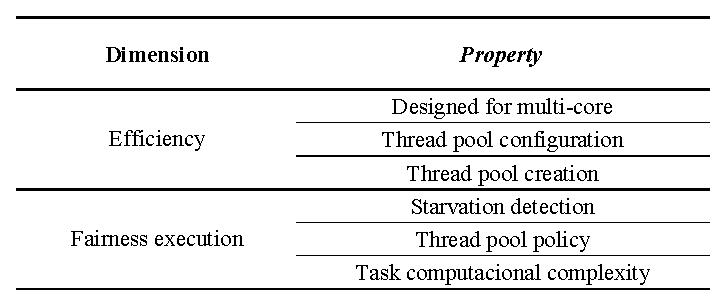
\includegraphics[scale=0.9]{./figs/issues.eps}
	%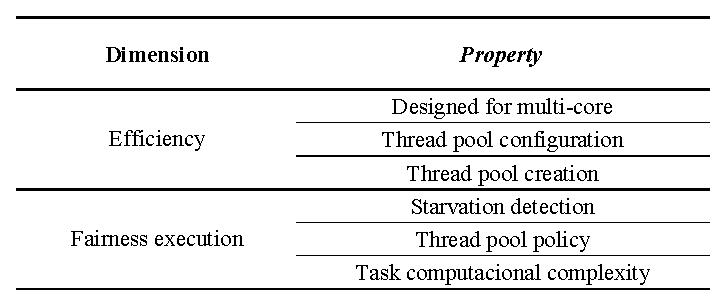
\includegraphics[width=\linewidth]{./figs/issues.eps}
\label{tab:problems}%
\end{table}%

%==============================================================================
\section{{Directions on Efficiency}}
\label{sec:directions_efficiency}
%==============================================================================
Software engineers seek to develop algorithms that can take full advantage of multi-core design so that achieve a high level of parallelism and an overall high performance. The way the algorithms are written impact in the success of multi-core technology strongly~\cite{sethi2015}. Design multi-core is a property, which should be present in runtime systems bearing in mind that the technological advances already offers resources to extends the parallel program. For hardware, modern technologies as Graphics processing units (GPUs) can be cited, which demand tens of thousands of concurrent threads to fully utilize the massive amount of processing resources~\cite{yoon2016}. GPUs hold great massively parallel computing capabilities, with potential for the acceleration of computationally intensive algorithms~\cite{tang2017}. 

Some works are shown promising proposals of thread pool configuration models, like the article of Nazeer et al.~\cite{nazeer2016}, which achieves good results in simulations, with the named Hybrid scheme to dynamically, which optimize a thread pool, based on predicting incoming request frequencies. Gleyzer et al.~\cite{gleyzer2017} propose a method allows dynamic thread pool sizing suitable for use in multi-threaded processing environment such as a distributed data grid. The method utilizes measurements of thread pool throughput and measurements of worker thread utilization in combination with analysis of prior thread pool resizing actions to determine whether to add or remove worker threads from a thread pool in a current resizing action. The method claims a rapid and responsive adjustment of thread pool size in response to changes in workload and processor availability. These works motivate us to deepen our research, so that the thread pool configuration of the runtime systems of the integration platforms occurs elastically, following the demand of processing the tasks and thus, using the computational resources more efficiently.

The research of Lee et al.~\cite{lee2011} shows better response time and CPU usage, by means prediction of the number of threads and thread pool management. Trendy exponential moving average (TEMA) scheme, proposed by Lee et al., adjusts the idle time out period and thread pool size to adapt the system to the changing environment. The article of Oh and Kim~\cite{oh2013} presents a history-based dynamic method (HisDyn), which minimizes throughput degradation, due to creation of threads, by means of estimation and maintenance of the number of threads needed for requests. HisDyn predicts the range of needed threads, through of the mean task arrival times and mean task processing times.

Bahadur et al.~\cite{bahadur2014} propose a thread pool system able of dynamic optimization thread pool size, according request frequencies, named Frequency Based Optimization Strategy (FBOS). After, Ashraf et al.~\cite{ashraf2016} present an extension of work of FBOS, namely Non-blocking Frequency Based Optimization Strategy with Automated Timers (NBFBOS with Automated Timers), which dynamically optimises thread pool, using of non-blocking synchronization primitives offering advantages of substantial scalability and liveliness. For all this, it is possible to find out to get optimised strategies to create threads at runtime to runtime systems of integration platforms.

%==============================================================================
\section{{Directions on Fairness Execution}}
\label{sec:directions_fairness}
%==============================================================================
Shah et al.~\cite{shah2017} argue that when starvation occurs it decreases response time and increases wait time to execution of requests and propose to explore the implementation of multiple thread pools based on a distribution of service times to avoid starvation and achieve concurrency of processing. Their analysis showed that proposed scheme is increases the response time and reduces the wait time. This research endorses the need and possibility of the runtime systems detecting starvation detection, therefore, the detection starvation is a potential field of study.

Tsai et al.~\cite{tsai2013} propose to optimize task scheduling and resource allocation using an improved differential evolution algorithm (IDEA), based on the proposed cost and time models on cloud computing environment. Elmougy et al.~\cite{elmougy2017} propose a novel hybrid task scheduling algorithm named (SRDQ) combining Shortest-Job-First (SJF) and Round Robin (RR) schedulers considering a dynamic variable task quantum. Singh et al.~\cite{singh2017} present a review of using meta-heuristics techniques for scheduling tasks in cloud computing, based on swarm intelligence and bio-inspired techniques and claim that it is possible to decide suitable approach for better schemes for scheduling according to the application. These works encourages us to pursue smarter policies to schedule tasks for the thread pools in the runtime systems of integration platforms.

Cordes et al.~\cite{cordes2011} claim that it is essential to balance the execution time of all tasks in a work flow of processing running in parallel in order to achieve the best possible utilization of computing resources. The proposed method by authors employs a cost model that allows incorporating differing execution times for loop iterations of the program due to the underlying heterogeneous platform. The consideration of execution time heterogeneity enables the in parallel approach to using each processing unit according to its performance characteristics in a system as well as the utilization of as many processing units as possible simultaneously.

Sudarsanam et al.~\cite{sudarsanam2004} address the compatibility between resource and task by estimating the amount of resources that are needed for a reconfigurable architecture to suit task granularity. These studies point out that considering the computational complexity to be executed can lead to a better allocation of computational resources.

% Capítulo 5:
\chapter{VALIDATION}
%capitulo09
\label{cap:validation}
\noindent 
This section indicates how the proposal will be validated by means whose the solutions found for the implementation of a more efficient runtime system will be validated. We will carry out experiments with the execution of business process integration solutions in different runtime systems. The results of these experiments will be used to analyse and compare the performance of the runtime systems. It will be considered the best performance runtime system, the one that has the lowest total average processing time of a message in the flow of an integration solution, considering the same message input rate and using the same amount of computational resources, amount of threads and memory, for each of the runtime systems tested.

According to the Law of Large Numbers~\cite{hoeffding1961}, in a performance comparison of execution of applications between runtime systems, when the number of performance observations is infinite, then the performance distribution of each runtime system, as well as its quantitative features, can be accurately captured, becoming this comparison straightforward and accurate. However, in practice, the number of collected performance observations is limited, then it is necessary to introduce a quantitative indicator of confidence to judge whether a comparison result corresponds to a stochastic effect or whether it is significant enough to accept.

Usually, estimating confidences of performance evaluations use parametric statistic \textit{t}-statistics. However, in the context of runtime system performance, \textit{t}-statistics require the sample mean of the performance observations to be distributed normally, which must be guaranteed by either a normal performance distribution or a sufficiently large number of performance observations~\cite{sitthi2006}. For validation of the proposed runtime system, it will be used the Hierarchical Performance Testing (HPT) framework~\cite{chen2015}, based on non-parametric statistics, which provide a good quantitative estimate of the confidence and it is significantly more practical than standard \textit{t}-statistics, because it does not require to collect a large number of performance observations in order to achieve a normal distribution of sample mean. 
% %==============================================================================
% \subsubsection{Qualitative performance comparisons non-parametric HPT framework}
% \label{subsubsec:qualitative}
% %==============================================================================
% In HPT, performance samples of a runtime system $X$ and of a runtime system $Y$ can be represented by performance matrices $S_{X}={\left [ x_{i,j} \right ]}_{m \ast n}$ and $S_{Y}={\left [ y_{i,j} \right ]}_{m \ast n}$, respectively, where $n$ is a total number benchmark applications and $m$ is a total number of repetitions of execution of the application. So, the performance scores of $X$ and $Y$ at their $j-th$ runs on the $i-th$ benchmark is $x_{i,j}$ and $y_{i,j}$ respectively. For the corresponding rows of $S_{X}$ and $S_{Y}$.
% HPT establishes as the null hypothesis and the alternative hypothesis of Statistical Hypothesis Test (SHT):
% \begin{description}
% \item [Null hypothesis $H_\tau,0$]: \textit{the performance scores of $X$ and $Y$ on the $\tau-th$ benchmark are equivalent to each other}
% \item [Alternative hypothesis $H_\tau,1$]: \textit{the performance score of $X$ is higher than that of $Y$ on the $\tau-th$ benchmark}
% \end{description}
% The Wilcoxon Rank-Sum Test\cite{wilcoxon1992} is used to investigate whether the difference between the performance score of $X$ and $Y$ is significant enough. The steps of Wilcoxon Rank-Sum Test are described as following:
% \begin{itemize}
% \item Define the significance level be $\alpha _{\tau }$ , where the literature suggests setting $\alpha _{\tau }$ = 0.05 for $m$ ≥ 5 and 0.10 for the rest cases.
% \item Sort $x _{\tau,1}$, $x _{\tau,2}$,...,$x _{\tau,m}$, $y _{\tau,1}$, $y _{\tau,2}$,...,$y _{\tau,m}$ in ascending order, and assign each of the scores the corresponding rank , from 1 to 2$m$. The rank sums of $X$ and $Y$, on the $\tau-th$ benchmark, are defined as:
% \[ R_{X,\tau }=\sum_{j=1}^{m}Rank_{\tau}\left ( x_{\tau ,j} \right ), R_{Y,\tau }=\sum_{j=1}^{m}Rank_{\tau}\left ( y_{\tau ,j} \right ),\]
% where $Rank_{\tau}\left ( . \right )$ provides the rank of a performance score on the $\tau-th$ benchmark.
% In statistics, when $m < 12$, the critical values for Wilcoxon rank sum test are calculated directly. When $m\geq 12$, the corresponding critical values are often estimated by studying the approximate distribution of the rank sum.
% \item Case $m < 12$, when the alternative hypothesis of the SHT is $H_\tau,1$], the null 		hypothesis is rejected and $H_\tau,1$ is accepted,if $R_{x,\tau }$, is no smaller than the critical value under the significance level $\alpha _{\tau }$~\cite{hogg2009}.
%  \item Case $m\geq 12$, define two new statistics $z _{x,\tau }$. and $z _{y,\tau }$ as follows:
% \[ z_{X,\tau}=\frac{R_{X,\tau}-\frac{1}{2}m\left (2m+1 \right )}{\sqrt{\frac{1}{12}m^2\left ( 2m+1 \right )}}, z_{Y,\tau}=\frac{R_{Y,\tau}-\frac{1}{2}m\left (2m+1 \right )}{\sqrt{\frac{1}{12}m^2\left ( 2m+1 \right )}}\]
% Under the null hypothesis, $z_{X,\tau}$, and $z_{Y,\tau}$, approximately obey the standard normal distribution $\mathit{N}\left (0,1 \right )$. When the alternative hypothesis of the SHT is $H_\tau,1$, the null hypothesis is rejected and $H_\tau,1$ is accepted, if $z_{x,\tau}$ is no smaller than the critical value under the significance level $\alpha _{\tau }$~\cite{hogg2009}.
%
% After carrying out the above SHT with respect to the $\tau-th$ benchmark $\left ( \tau = 1, . . . , n\right )$, it is possible to assign the difference, denoted by $d-\tau$, between the performance of $X$ and $Y$. If the SHT accepts $H_\tau,1$ with a significance level between 0.01 and 0.05, then
% \[d_{\tau} = median\left \{ x_{\tau ,1}, x_{\tau ,2},...,x_{\tau ,m} \right \}- median\left \{ y_{\tau ,1}, y_{\tau ,2},...,y_{\tau ,m} \right \}, \tau = 1,..,n.
% \]
% Otherwise, when the null hypothesis $H_\tau,0$ has not been rejected at a promising significant level, $d_\tau = 0$, the insignificant difference between the performance scores of $X$ and $Y$ is ignored.
% $d_1, d_2, . . . , d_n$ will then be utilized in the following Wilcoxon Signed-Rank Test~\cite{wilcoxon1992} for the performance comparison over different benchmarks.
% \end{itemize}
%
% In case that there are not significant difference between the performance scores of $X$ and $Y$, HPT establishes as the null hypothesis and the alternative hypothesis of Statistical Hypothesis Test (SHT):
% \begin{description}
% \item [Null hypothesis $H_0$]: \textit{the general performance of $X$ is equivalent to that
% of $Y$}
% \item [Alternative hypothesis $H_1$]: \textit{the general performance of $X$ is better than that of $Y$}
% \end{description}
% The Wilcoxon Signed-Rank Test~\cite{wilcoxon1992} is used to calculate the critical value under
% the significance level, as following:
% \begin{itemize}
% \item Rank $d _1$, $d _2$,...,$d _n$ according to an ascending order of their absolute values. The rank sums of $X$ and $Y$, on the signed-rank sums are defined as:
% \[ R_X=\sum_{i:d_i>0}Rank\left ( d_i \right ) + \frac{1}{2} \sum_{i:d_i=0}Rank\left ( d_i \right ), R_Y=\sum_{i:d_i<0}Rank\left ( d_i \right ) + \frac{1}{2} \sum_{i:d_i=0}Rank\left ( d_i \right )\],
% where $ Rank \left ( d_i \right) $ provides the rank of absolute value of the $d_i$.
%
% In statistics, when $n < 25$, the critical values for Wilcoxon Signed-Rank Test are calculated directly, otherwise, when $n\geq 25$, the corresponding critical values are often estimated by studying the approximate distribution of the signed rank sum. 
% \item Case $n <25$, when the alternative hypothesis of the SHT is $H_1$, the null hypothesis is rejected and $H_1$ is accepted, if $R_Y$ is no larger than the critical value under the significance level~\footnote[1]{The critical values of Wilcoxon Signed-Rank Test are available in statistics books~\cite{hogg2009} } $\alpha$.
% \item Case $n\geq 25$, two new statistics $z_X$ and $z_Y$ are defined:
% \[ z_{X}=\frac{R_{X}-\frac{1}{4}n\left (n+1 \right )}{\sqrt{\frac{1}{24}n\left ( n+1 \right ) \left ( 2n+1 \right )}},
%  z_{Y}=\frac{R_{Y}-\frac{1}{4}n\left (n+1 \right )}{\sqrt{\frac{1}{24}n\left ( n+1 \right ) \left ( 2n+1 \right )}} \]
%  Under the null hypothesis, $z_X$, and $z_Y$, approximately obey the standard normal distribution $\mathit{N}\left (0,1 \right )$.
 %
% Hence, when the alternative hypothesis of the SHT is $H_1$, the null hypothesis is rejected and $H_1$ is accepted, if $z_Y$ is no larger than the critical value under the significance level $\alpha$. For the comparison over different benchmarks, the outputs of the HPT, including the comparison result and its confidence, are finally presented by the above Wilcoxon Signed-Rank Test. Formally, given a fixed significance level $\alpha$ for the HPT, the assert made by the HPT: \textit{X outperforms Y with the confidence $r$}, where $r = 1 - \alpha$ is represent by $ Confidence(\textsc{HPT} : S_X\succ S_Y)\geq r $.
%  \end{itemize}
 %
% %==============================================================================
% \subsubsection{Quantitative performance comparisons non-parametric HPT framework}
% \label{subsubsec:quantitative}
% %==============================================================================
%
% In most cases, there is more interest in quantitative comparison results such as “Runtime system X is more than $\gamma$ times faster than runtime system Y”, where $\gamma \geq 1$ is defined as the speedup-under-test. The HPT framework provides provides two approaches speedup arguments: \textit{(i)} requires a previously value for $\gamma$ and \textit{(ii)} requires the largest speedup that results in a reliable comparison result.
%
% The first approach requires a previously value for $\gamma$. Afterwards, the performance scores of runtime system X are shrieked by transforming the corresponding performance matrix $S_X$ to $\frac{S_X} {\gamma} $, without losing generality, it is employed normalized performance ratio as performance score with respect to each benchmark, where a larger performance score means better performance. Considering a virtual runtime system with performance matrix $S_X$ to $ \frac {S_X}  {\gamma} $, if the HPT framework states that the virtual runtime system outperforms runtime system Y with a confidence $r$, it is possible to claim \textit{X has a performance times better $ \gamma $ than Y with a confidence $r$ }. In general, if a more conservative speedup is specified before speedup testing, the corresponding speedup argument will have a larger confidence $r$; otherwise, if a less conservative speedup is specified before speedup testing, the corresponding speedup argument will have a smaller confidence $r$. Chen et al.~\cite{chen2015}, HPT authors, recommend to keep a balance between the speedup and the corresponding confidence, so as to make a convincing yet not-too-conservative conclusion.
%
% When the interest is to know the largest speedup that results in a reliable comparison result, for a given confidence $r$. For this approach, HPT framework offers an alternative way of estimating the speedup and corresponding confidence, defining the $r$-Speedup as:
% \[ 
% \texttt{sup}\left \{ \gamma \geq 1;confidence\left ( \textsc{HPT}:\frac{1}{\gamma}S_X \succ S_Y \right )\geq r\right \}
% \]
% Then, the $r$-Speedup of runtime system X over runtime system Y is the largest speedup of X over Y having a confidence above $r$ . The $r$-Speedup can be  viewed as a quantitative indicator of performance speedup with the guarantee of confidence $r$ and, therefore, it can also act as a single-number performance metric.
%\textbf{Variables}

The variables in the statistical studies are the values that assume certain characteristics of interest for research. The following are the variables from which we will extract the values in several scenarios in order to analyse the performance of the compared execution engines. The variables studied are classified as continuous quantitative variables, since they assume numerical values that vary within an infinite range, with the exception of variable 5, which is classified as discrete quantitative, since it assumes only integer and positive numerical values.
\begin{enumerate}
\item Average total CPU time per task.
\item Total average wait time for tasks in the task queue.
\item Total average processing time of tasks.
\item Average total bytes processed per unit of time.
\item Average number of messages processed per unit of time.
\item Average total CPU time in processing a message.
\end{enumerate}
% \noindent
% \textbf{Treatment Factor 3 x 3 x 3}
In an experiment, the factor, also called an independent variable, is an explanatory variable manipulated by the experimenter. The different values of the factor are called \textit{level} and the combinations of factor levels are called \textit{treatments}. In our case, we will have the following treatment factors: \textit{(i)} Runtime systems execution models, textit{(ii)} Integration solution and textit{(iii)} Message input rate. First factor is classified as nominal qualitative and its levels will be: task-based, process-based, proposed model. Second factor is classified as qualitative and its levels will be different integration solutions to be defined. Latter is classified as continuous quantitative and its levels will be message input rates to be defined.
% These factors are classified as qualitative, when it assumes non-numerical and quantitative values when it assumes numerical values. The treatment factors of our statistical validation model and their respective levels are listed below. 
% \begin{itemize}
% \item Treatment Factor 1
%     \begin{itemize}
%       \item Type: Nominal Qualitative.
%       \item Description: Integration platforms runtime systems models.
%       \item Levels: task-based $(M_1)$, process-based$(M_2)$, proposed model$(M_3)$.
%     \end{itemize}
% \item Treatment Factor 2
%     \begin{itemize}
%     	\item Type: Qualitative.
%     	\item Description: Solution for integrating enterprise processes in cloud computing.
%     	\item Levels: Three different solution for integration to be defined $(S_1,S_2,S_3)$.
%     \end{itemize}
% \item Treatment Factor 3
%     \begin{itemize}
%     	\item Type: Continuous quantitative.
%     	\item Description: Message input rate, set of bytes per second.
%     	\item Levels: Three different message input rates, set of bytes per second to be defined $(R_1,R_2,R_3)$.
%     \end{itemize}
% \end{itemize}

% The experiment is classified as \textit{Mixed} in relation to the factors: \textit{runtime system model}, \textit{integration solution} e \textit{input rate} and it has a total of 27 experimental units, as shown in Table~\ref{tab:factors}.

% \begin{table}[!htb]
% \centering
% \caption{Relation to the factors}
% \label{tab:factors}
% \begin{tabular}{lllcclllcclll}
% \hline
% $M_1$ & $S_1$ & $R_1$ & & & $M_2$ & $S_1$ & $R_1$  & & & $M_3$ & $S_1$ & $R_1$ \\ \hline
% $M_1$ & $S_1$ & $R_2$ & & & $M_2$ & $S_1$ & $R_2$  & & & $M_3$ & $S_1$ & $R_2$ \\ \hline
% $M_1$ & $S_1$ & $R_3$ & & & $M_2$ & $S_1$ & $R_3$  & & & $M_3$ & $S_1$ & $R_3$ \\ \hline
% $M_1$ & $S_2$ & $R_1$ & & & $M_2$ & $S_2$ & $R_1$  & & & $M_3$ & $S_2$ & $R_1$ \\ \hline
% $M_1$ & $S_2$ & $R_2$ & & & $M_2$ & $S_2$ & $R_2$  & & & $M_3$ & $S_2$ & $R_2$ \\ \hline
% $M_1$ & $S_2$ & $R_3$ & & & $M_2$ & $S_2$ & $R_3$  & & & $M_3$ & $S_2$ & $R_3$ \\ \hline
% $M_1$ & $S_3$ & $R_1$ & & & $M_2$ & $S_3$ & $R_1$  & & & $M_3$ & $S_3$ & $R_1$ \\ \hline
% $M_1$ & $S_3$ & $R_2$ & & & $M_2$ & $S_3$ & $R_2$  & & & $M_3$ & $S_3$ & $R_2$ \\ \hline
% $M_1$ & $S_3$ & $R_3$ & & & $M_2$ & $S_3$ & $R_3$  & & & $M_3$ & $S_3$ & $R_3$ \\
% \end{tabular}
% \end{table}

% Capítulo 6:
\chapter{SCHEDULE AND CURRENT STAGE}
%capitulo08
\label{cap:schedule}
\noindent 

This section presents the schedule of activities for the development of this doctoral research project, starting in April of 2016 and ending in March 2020, totalling a period of 48 months. The dependence between the steps can lead, at some point, to changes in the schedule, and its restructuring is necessary. The activities of the nearest steps have a more detail level than those of the later steps, which are in a higher level of abstraction, because, as discussed in Section~\ref{cap:methodology}, with each step start, there is a planning in which discussed and listed the next activities and artefacts produced.
The focus of research from the present moment will be on the choice of approach to the research problems described in  Section~\ref{cap:researchproblems}.
Table~\ref{tab:schedule1} presents the planning of the academic training activities and the planning of the research activities.

\begin{table*}[htbp]
	\centering
	\caption{Schedule of activities.}
    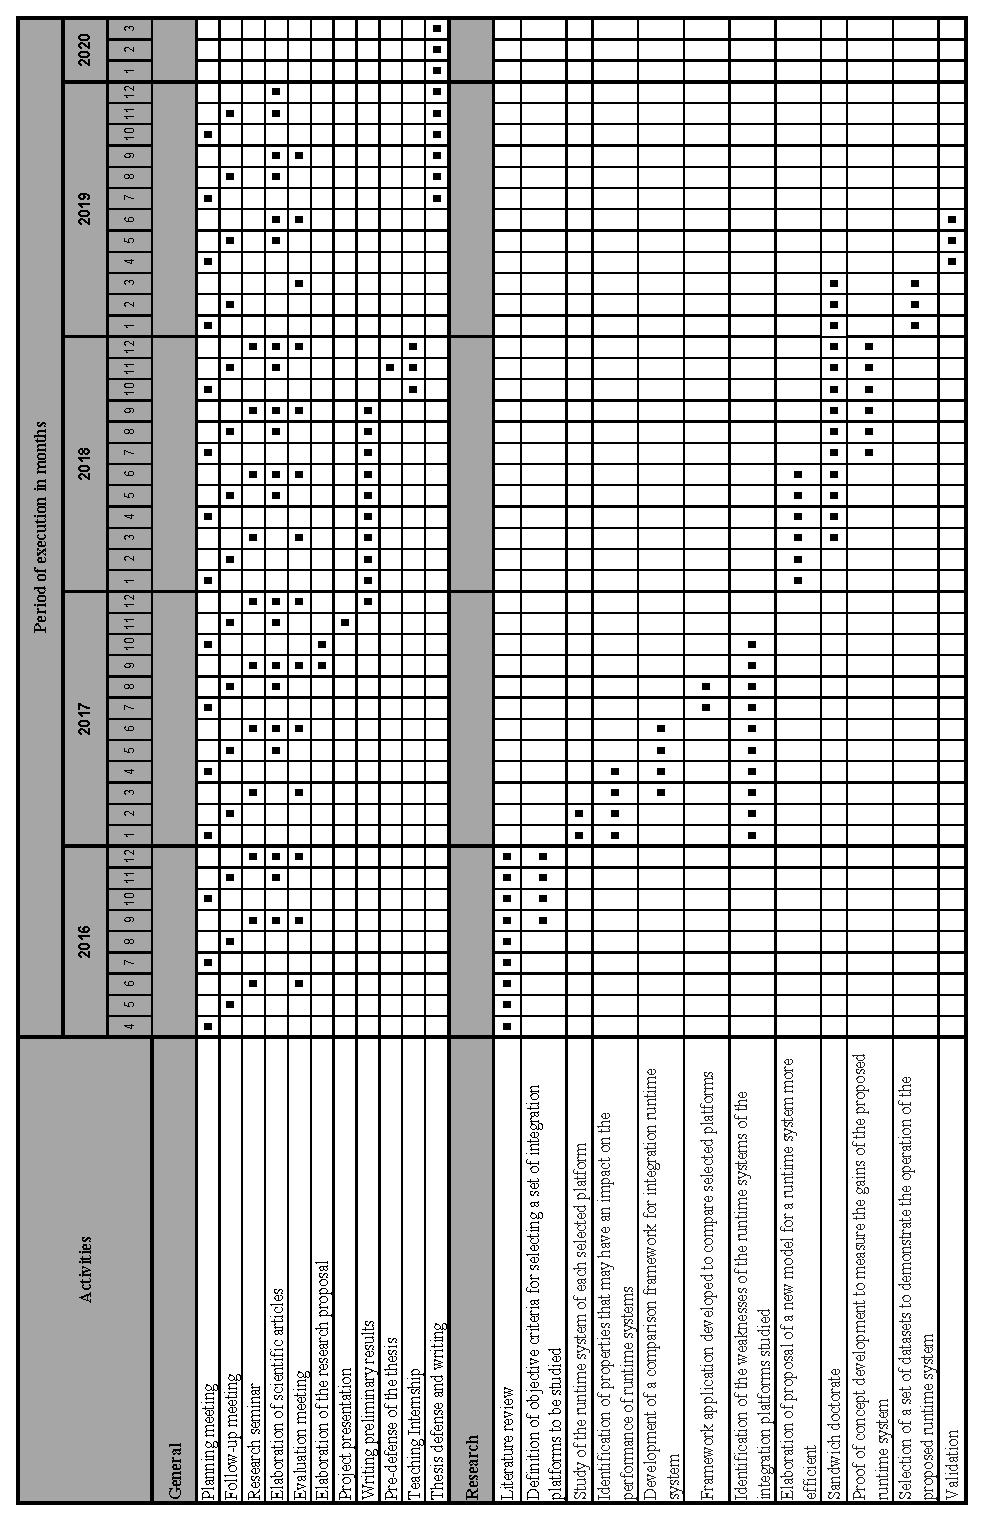
\includegraphics[scale=0.95]{./figs/schedule.eps}
	%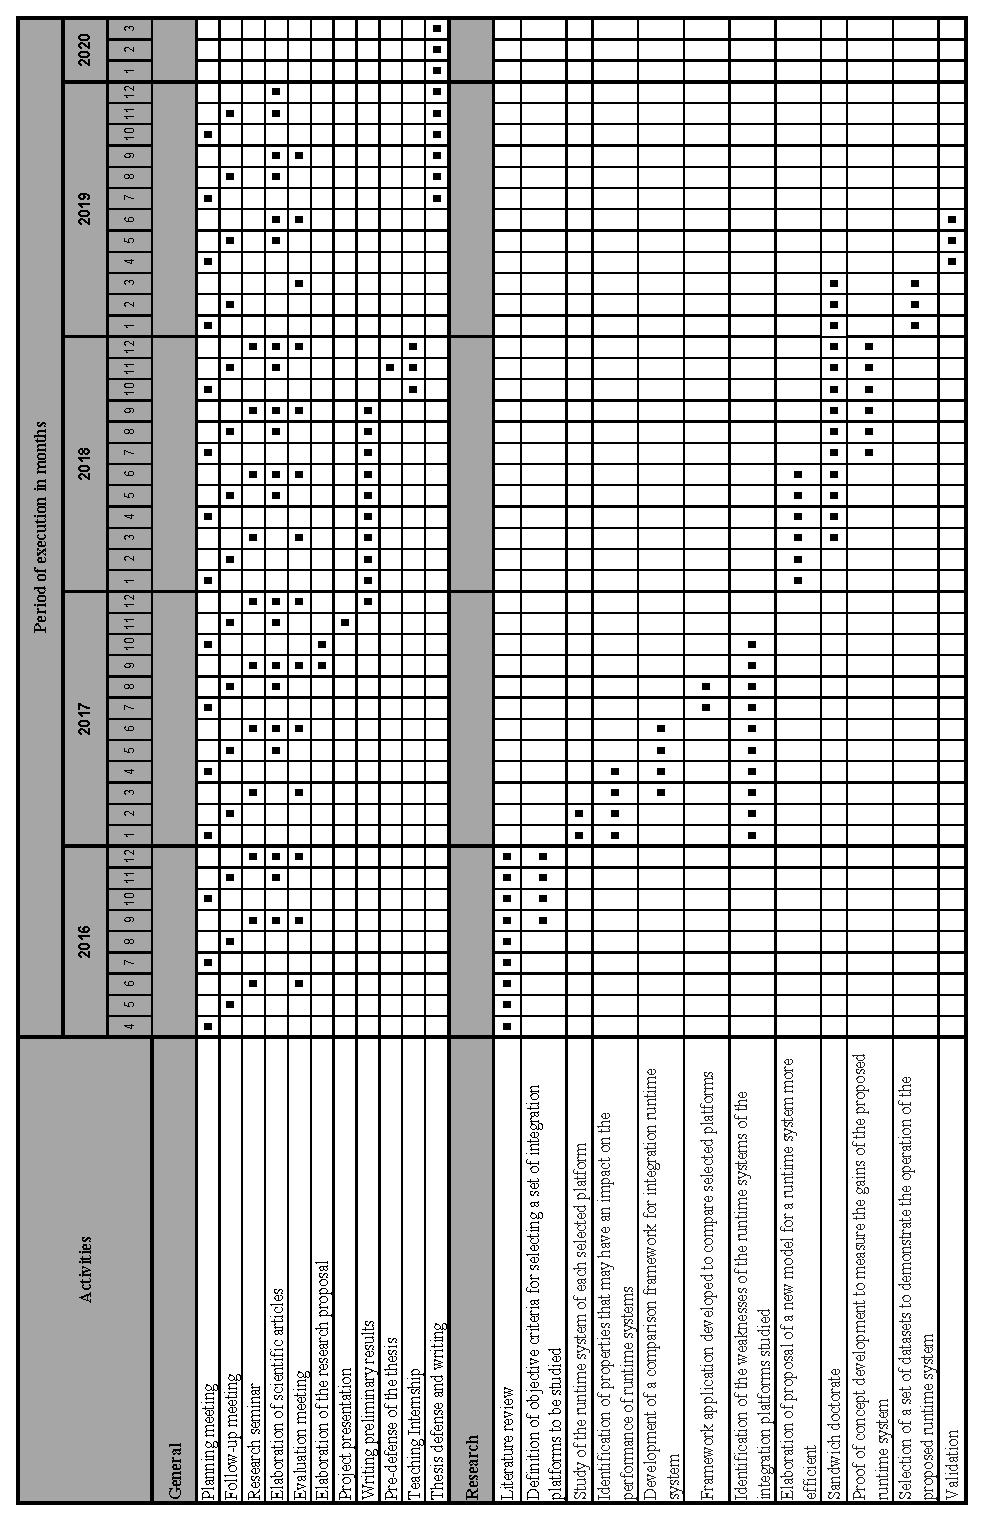
\includegraphics[width=\linewidth]{./figs/schedule.eps}
	\label{tab:schedule1}
\end{table*}

%current stage
In the first year of the research, we studied o research context, including EAI, runtime system, cloud computing and big data. After, we did a deep literature review in order to expand knowledge in the research fields: mathematical modelling, optimization techniques, statistics models and multithread programming. These knowledge form the foundation of our research.
Parallel, we determined criteria for selecting a set of integration platforms to be studied.

From the second year of research, we studied the runtime system of the selected platform e found properties that may have an impact on the performance of runtime systems. With that, we can development of a comparison framework for integration runtime system and apply it in the comparison of platforms, and finally, identified weaknesses of the runtime systems. The result generated a partial technical report. During this period, we produced peripheral works, which can lead or contribute to the solutions to the research questions.

We are begging a step third of research that is an elaboration of a proposal of a new model for a runtime system more efficient.

% Capítulo 5:
\chapter{AVAILABLE INFRASTRUCTURE}
%capitulo05
\label{cap:infrastructure}
\noindent
The project will be developed in the Laboratory of Applied Computing,under coordination of GCA, in Department of Exact Sciences and Engineering, Uniju\'{i} University. The laboratory is installed in a research room with approximately 45 $m^2$.

For tasks that require less processing power, such as: literature review, production of scientific articles, elaboration of algorithms and other artefacts of the research,  will be used a computer, which has the following configuration: operational system Microsoft Windows 10 Education, Intel(R) Core(TM) i5-5200U CPU, 2.20GHz; 2195 Mhz, 2 Cores(s), 4 logical processors, memory RAM of 4.00 GB.

The simulation of mathematical models and the high performance computational experimentations will to be carry out a server, which has the following configuration: storage SAS of 6 Gb, 12 units of 2U, two cache controllers of 4 GB; six discs of 2TB, 2.7 K rpm, NLSAS 12Gbps; our Intel Xeon E5-4610 v4 1.8GHz cache of 25M, QPI of 6.4 GT/s, without turbo, HT, ten cores/twenty segments; three SAS 2.5", 12Gbps 300GB disks; twenty four 16 GB RDIMM memory combs, 2400 MT/s; RAID5 with three to six discs; two redundant power supplies.
% \begin{itemize}
%   	\item storage SAS of 6Gb, 12 units of 2U, two cache controllers of 4GB
%   	\item six discs of 2TB, 2.7K rpm, NLSAS 12Gbps
% 		\item four Intel Xeon E5-4610 v4 1.8GHz cache of 25M, QPI of 6.4 GT/s, without turbo, HT, ten cores/20 segments
% 		\item three SAS 2.5", 12Gbps 300GB Disks
% 		\item twenty four 16GB RDIMM memory combs, 2400 MT/s
% 		\item RAID5 with three to six discs
% 		\item two redundant power supplies
% \end{itemize}
In addition, for both internal meetings and specialized seminars, the Postgraduate Program in Mathematical Modelling of UNIJUÍ University offers: eight classrooms equipped with projectors, six laboratories with a total of 150 computers, meeting and study rooms and auditorium.

As technical support, the postgraduate program has two secretaries and two computer technicians who are in charge of the management and maintenance of the laboratories. The library of UNIJUÍ has several materials, ranging from books, magazines, catalogues, technical projects, to articles, dissertations and doctoral thesis; and it has a set of reading rooms where access to the internet is allowed.




% % Capítulo 6:
% \chapter{COLLABORATIONS}
% \input{src/collaboration.tex}
%
% % Capítulo 7:
% \chapter{CURRENT STAGE}
% \input{src/currentstage.tex}
%
%
% Referências bibliográficas:
\bibliography{bibliografia}

\end{document}
